\section{Introduction}
\label{sec:ai}


OpenAI are the creators of one of the most popular artificial intelligent (AI) chatbots called ChatGPT. ChatGPT is an artificial intelligence language model (LLM). An LLM is a program that can recognize and generate text based on large sets of data. For example, you could ask an LLM who won the 2022 FIFA world cup, and if it was trained well enough, the LLM would respond with Argentina. 
   
LLMs are trained on mass amounts of text in order to learn through a process called machine learning. Through machine learning an AI is able to develop without the need of direct human instruction. After feeding an LLM enough data it will start to be able to interpret and recognize the similarities between all of the data. Therefore giving it the ability to construct sentences properly, and answer questions that were within the data \citep{ChatGPT-functions} \cite{LLM}.

\begin{figure}[h]
  \centering
  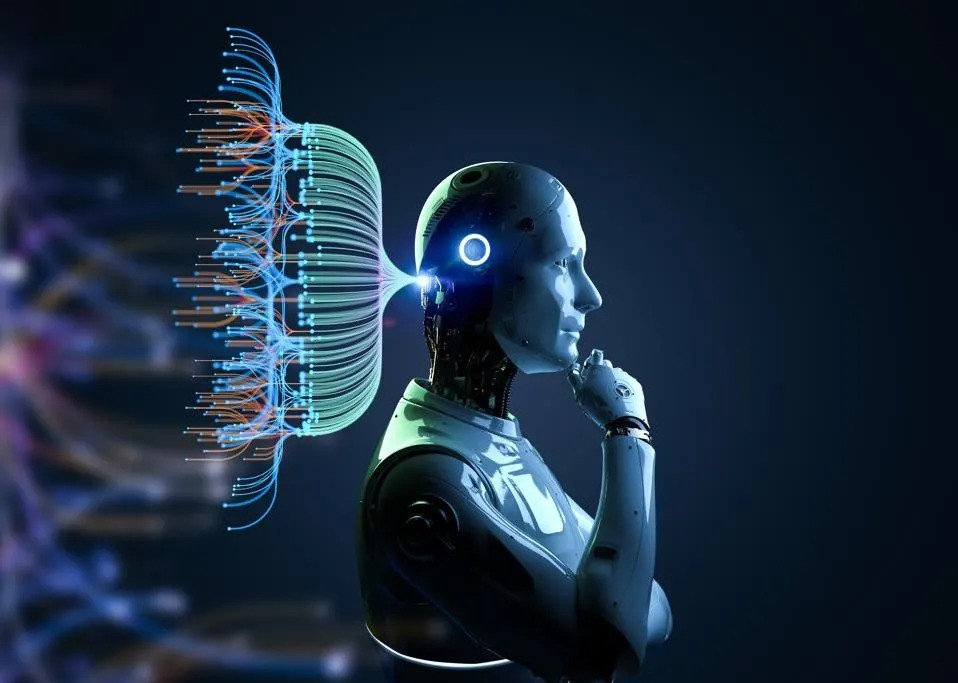
\includegraphics[width=0.5\textwidth]{E.jpg}
  \caption{Photo of AI - Getty Images}
  \label{fig:}
\end{figure}